\changecolours{ScoutGreen}
\section{A Importância do Cache, Expiração e Práticas de Atualização}

% ------------------------------------------------------------------------------
\twocolframe[title={Por que o Cache DEVE ser Expirável (TTL)?},leftcol=7cm,rightcol=7cm]{%
  \alert{1. A Finitude Física da Memória RAM}\par
  \itemseps[topsepi=2mm,itemsepi=3mm,labelsep=2mm,leftmargini=4mm]
  \begin{itemize}
    \item A memória RAM custa significativamente mais por gigabyte que discos NVMe.
    \item Se gravarmos todas as buscas e consultas no Redis sem expiração, a RAM esgotará rapidamente.
    \item \textbf{Políticas de Evicção:} Quando atinge o \texttt{maxmemory}, o Redis descarta chaves via algoritmos LRU (\textit{Least Recently Used}) ou LFU (\textit{Least Frequently Used}).
  \end{itemize}
}{%
  \alert{2. Autocura Contra Dados Obsoletos}\par
  \itemseps[topsepi=2mm,itemsepi=3mm,labelsep=2mm,leftmargini=4mm]
  \begin{itemize}
    \item Em arquiteturas distribuídas, sincronizações podem falhar por timeout de rede ou concorrência.
    \item \textbf{Self-Healing:} Um TTL bem calibrado (ex: 60s a 300s) atua como rede de segurança.
    \item Mesmo que a invalidação ativa falhe, a chave expira e a próxima consulta busca a verdade atualizada na fonte primária.
  \end{itemize}
}

% ------------------------------------------------------------------------------
\begin{frame}{Padrões de Atualização de Cache e Sincronização}
  \centering
  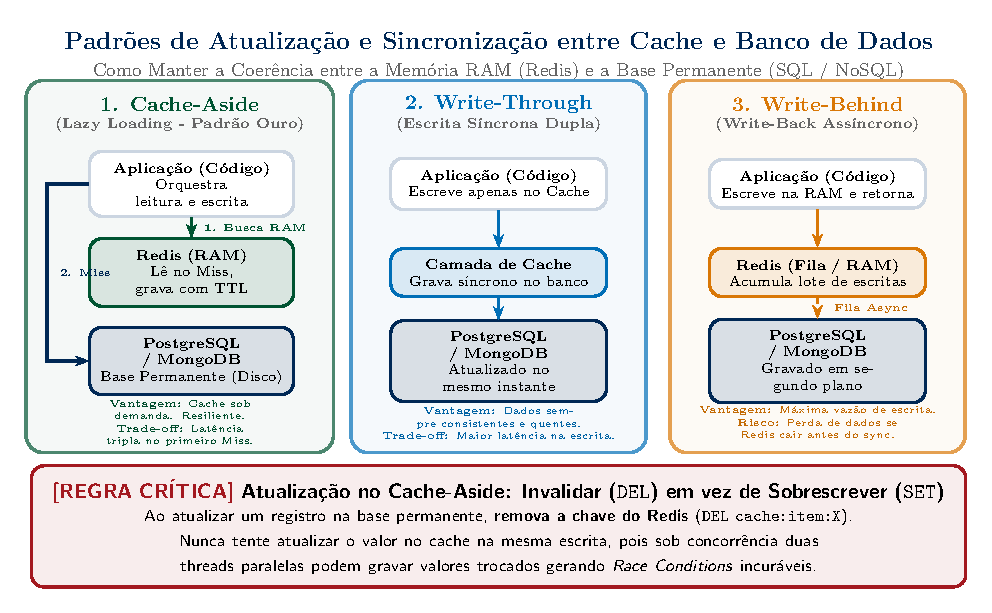
\includegraphics[width=0.90\textwidth,height=0.74\textheight,keepaspectratio]{figuras/fig_padroes_atualizacao.pdf}
\end{frame}

% ------------------------------------------------------------------------------
\twocolframe[title={Invalidação no Cache-Aside: O Risco de Race Conditions},leftcol=7cm,rightcol=7cm]{%
  \alert{O Erro Comum de Iniciante}\par
  \itemseps[topsepi=2mm,itemsepi=3mm,labelsep=2mm,leftmargini=4mm]
  \begin{itemize}
    \item Ao atualizar um produto no banco relacional, tentar atualizar o valor diretamente no Redis via \texttt{SET}.
    \item \textbf{Cenário de Desastre:} Sob alta concorrência, a Requisição 1 atualiza o SQL e depois a Requisição 2 atualiza o SQL.
    \item Porém, pela rede, o \texttt{SET} da Requisição 1 chega no Redis \textbf{depois} do \texttt{SET} da Requisição 2!
  \end{itemize}
}{%
  \alert{A Consequência Grave}\par
  \itemseps[topsepi=2mm,itemsepi=3mm,labelsep=2mm,leftmargini=4mm]
  \begin{itemize}
    \item O banco relacional permanente fica com o valor novo (da Requisição 2).
    \item O Redis fica com o valor velho (da Requisição 1) gravado para sempre!
    \item O cache torna-se inconsistente com a verdade do sistema.
  \end{itemize}
}

% ------------------------------------------------------------------------------
\begin{frame}[fragile]{Solução: A Regra de Ouro da Invalidação (DEL)}
  \begin{columns}[T]
    \begin{column}{0.48\textwidth}
      \alert{Invalidação Limpa e Segura}\par
      \itemseps[topsepi=1mm,itemsepi=1.5mm,labelsep=2mm,leftmargini=4mm]
      \small
      \begin{itemize}
        \item Ao alterar o banco permanente, \textbf{apenas delete a chave do Redis (\texttt{DEL})}.
        \item Não tente adivinhar o valor do cache na mesma escrita.
        \item A próxima leitura disparará \textit{Cache Miss}, recarregando a verdade da base SQL com novo TTL.
      \end{itemize}
    \end{column}
    \begin{column}{0.50\textwidth}
      \alert{Fluxo Seguro no Terminal}\par
      \begin{lstlisting}[language=bash]
# 1. Atualizar registro no banco SQL:
# UPDATE produtos SET preco=3599 WHERE id=101;

# 2. Invalidar imediatamente no Redis:
127.0.0.1:6379> DEL busca:item:101
(integer) 1

# 3. Proxima leitura busca no SQL e repovoa:
127.0.0.1:6379> SET busca:item:101 "3599" EX 300
OK
      \end{lstlisting}
    \end{column}
  \end{columns}
\end{frame}

% ------------------------------------------------------------------------------
\begin{frame}[fragile]{Políticas de Evicção de Memória sob Sobrecarga}
  \begin{columns}[T]
    \begin{column}{0.48\textwidth}
      \alert{Algoritmos no Limite de RAM}\par
      \itemseps[topsepi=1mm,itemsepi=1.5mm,labelsep=2mm,leftmargini=4mm]
      \small
      \begin{itemize}
        \item Ao atingir o limite \texttt{maxmemory}:
        \item \textbf{volatile-lru:} Descarta chaves com TTL menos acessadas recentemente (\textit{Recomendado para cache}).
        \item \textbf{allkeys-lru:} Descarta qualquer chave LRU.
        \item \textbf{noeviction:} Retorna erro em comandos de gravação quando a memória enche.
      \end{itemize}
    \end{column}
    \begin{column}{0.50\textwidth}
      \alert{Diretivas no redis.conf}\par
      \begin{lstlisting}[language=bash]
# Limite maximo de memoria para o Redis:
maxmemory 4gb

# Politica recomendada para camada de cache:
maxmemory-policy volatile-lru

# Inspecionar consumo de memoria no CLI:
127.0.0.1:6379> INFO memory
# used_memory_human:1.24M
      \end{lstlisting}
    \end{column}
  \end{columns}
\end{frame}

% ------------------------------------------------------------------------------
\begin{frame}{Comprovação Experimental: Benchmarking de Latência}
  \centering
  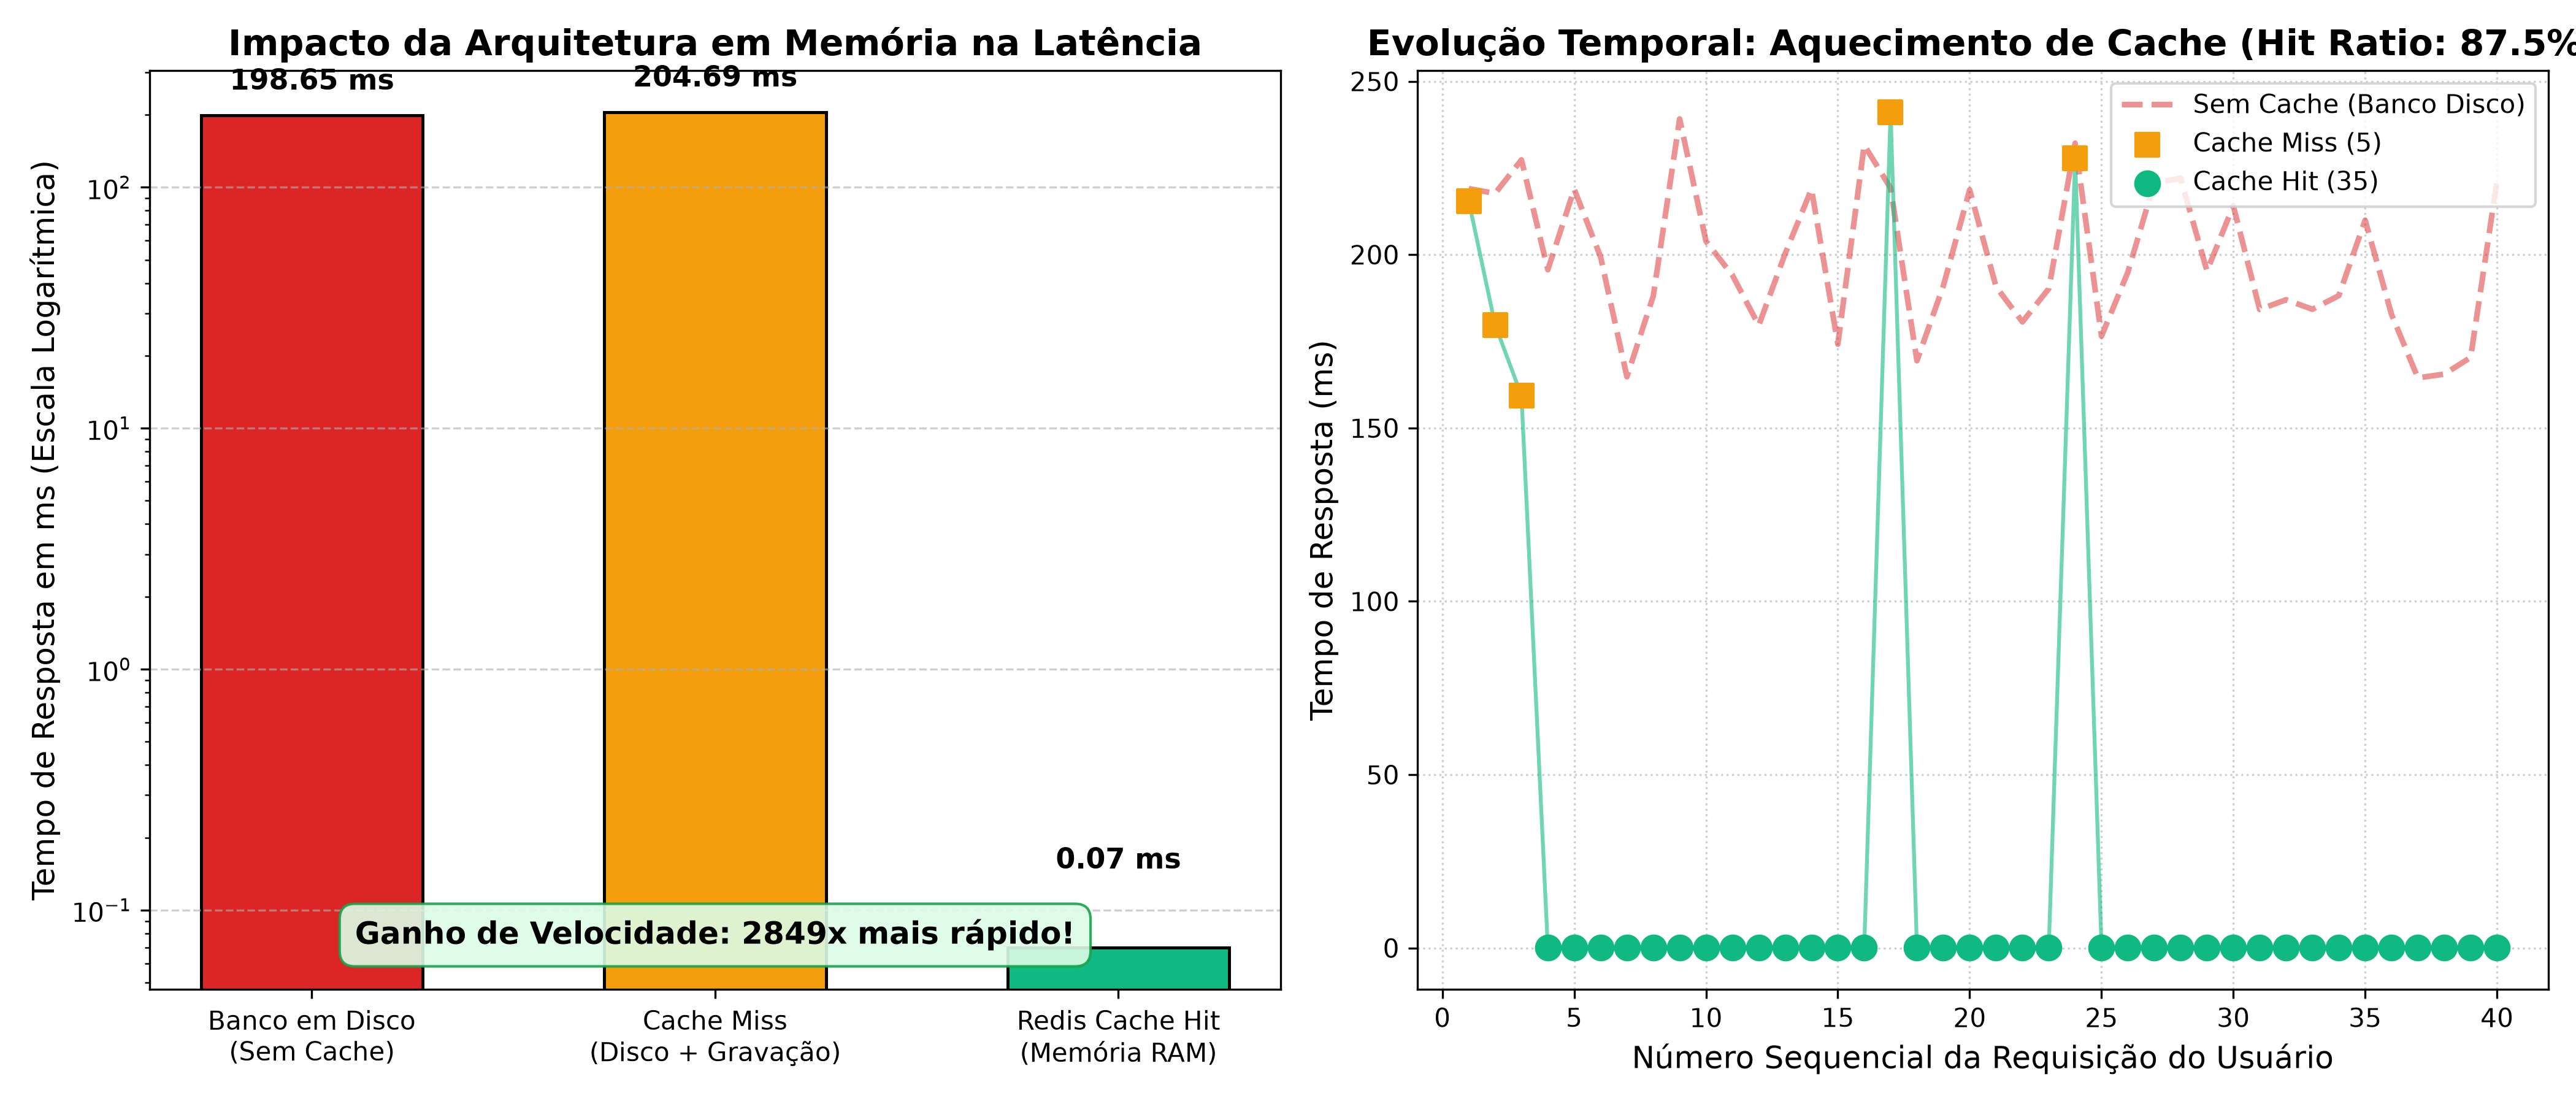
\includegraphics[width=0.88\textwidth,height=0.74\textheight,keepaspectratio]{figuras/grafico_latencia_busca.png}
\end{frame}
